\chapter{Modelos LW}


\section{\citet{LW:2003}:Measuring the Natural Rate of Interest }
A taxa natural de juros - a taxa de juros real de curto prazo consistente com produto, igualando sua taxa natural e inflação constante.

A taxa de juros real natural ou de "equilíbrio" fornece uma referência para medir a postura da política monetária, com a política expansionista (contracionista) se a taxa de juros de curto prazo estiver abaixo (acima) da taxa natural.

Abordamos essa questão calculando conjuntamente as taxas naturais de juros e produto e o crescimento da tendência nos últimos 40 anos de dados dos EUA, usando o filtro de Kalman. A taxa de juros natural mostra uma variação significativa nos últimos quarenta anos nos Estados Unidos, com a variação na taxa de crescimento tendencial sendo um importante determinante das mudanças na taxa natural, conforme previsto pela teoria. Esses resultados são robustos a mudanças na especificação. No entanto, as estimativas de uma taxa de juros natural variável no tempo, como aquelas das taxas naturais de desemprego e produção, são muito imprecisas e estão sujeitas a considerável mensuração em tempo real.

A taxa natural de juros está intimamente relacionada ao nível da taxa natural de produção, ela própria uma variável não observada. Da FOC do consumidor tem-se: 
\begin{equation}
    r = \dfrac{1}{\sigma} g_c + \theta
\end{equation}
$r$ é a taxa real de juros e $\sigma$ é a IES e $g_c$ a taxa de crescimento do consumo. Mudanças na taxa de crescimento tendencial nos Estados Unidos, sugerindo uma fonte de movimentos persistentes na taxa de juros natural; mudanças nas preferências e na política fiscal provavelmente contribuem também para a variação no tempo da taxa natural. Lei de movimento para taxa natural de juros, $r^{*}$:
\begin{equation}
    r_t^{*} = cg_t + z_t
\end{equation}
$g_t$ é a tendência de crescimento da taxa natural do produto e $z_t$ captura outros determinantes.

Os principais determinantes da taxa natural de juros não são observados, aplicamos o filtro de Kalman para estimar conjuntamente as taxas naturais de juros, produção e tendência de crescimento. A identificação econométrica da taxa natural de juros é obtida especificando-se uma equação IS de forma reduzida, em que o hiato do produto (o desvio percentual do PIB real da taxa natural de produção) é determinado por suas próprias defasagens, uma média móvel da defasagem da real-funds-rate gap (a diferença entre a taxa fed fund ex ante e $r^{*}$):

\begin{equation} \label{Eq_medida1}
    \tilde{y}_t = a_{y,1}\tilde{y}_{t-1} + a_{y,2}\tilde{y}_{t-2} + \dfrac{a_r}{2}\sum_{j=1}^{2} (r_{t-j} - r_{t-j}^{*}) + \varepsilon_{1,t}
\end{equation}

Supõe-se que a taxa de inflação seja determinada por suas próprias defasagens, o defasagem do produto, duas variáveis que medem a inflação dos preços relativos (choques de núcleo - importação excluindo petróleo, computadores e semicondutores) e inflação defasada do petróleo.

\begin{equation} \label{Eq_medida2}
    \pi_t = B_{\pi}(L)\pi_{t-1} + b_y \tilde{y}_{t-1} + b_i(\pi_t^{I} - \pi_t ) + b_{o}(\pi_{t-1}^{o} - \pi_t) + \varepsilon_{2,t}
\end{equation}

As eqs. (\ref{Eq_medida1}) e (\ref{Eq_medida2}) são as equações de medida da versão básica do modelo de espaço de estado. Há um versão amplificada que inclui horas trabalhadas:

\begin{equation}
    \tilde{h}_t = f_1\tilde{y}_t + f_2\tilde{h}_{t-1} + f_3\tilde{h}_{t-1} + \varepsilon_{6,t}
\end{equation}

$\tilde{h}_t$ é o desvio percentual entre as horas trabalhadas e a tendência log linear $h_t^{*}$.

Equações de Transição do modelo de espaço de estado:

\begin{equation}
    z_t = D_z(L)z_{t-1} + \varepsilon_{3,t}
\end{equation}

Permite choques para a taxa natural do produto e para a tendência do produto.

\begin{eqnarray}
    y_t^{*} = y_{t-1}^{*} + g_{t-1} + \varepsilon_{4,t} \\
    g_t^{*} = g_{t-1}^{*} + \varepsilon_{5,t}
\end{eqnarray}

Estima o modelo via máxima verossimilhança. Em duas etapas. Na primeira etapa, aplique o filtro de Kalman para estimar a taxa natural do produto, omitindo o termo do hiato da taxa real da equação (\ref{Eq_medida1}) e assumindo que a taxa de crescimento de tendência g é constante.
%
%
\section{\citet{HLW:2017}: Measuring the natural rate of interest: International trends and determinants}

Neste artigo, estendemos essa análise para outras economias avançadas. Estimamos uma versão do modelo de \citet{LW:2003} da taxa natural de juros, originalmente desenvolvida para a economia americana, usando dados de quatro economias: Estados Unidos, Canadá, Área do Euro e Reino Unido. Esse modelo aplica o filtro de Kalman a dados sobre o PIB real, a inflação e a taxa de juros de curto prazo para extrair componentes altamente persistentes da taxa natural de produção, sua taxa de crescimento tendencial e a taxa natural de juros.

Nossa análise produz quatro resultados principais. Primeiro, encontramos evidências de variação no tempo na taxa natural de juros em todas as quatro economias. Em segundo lugar, há uma tendência de queda nas taxas de juros naturais estimadas: No final de nossa amostra, as taxas naturais estimadas de juros nas quatro economias caíram para níveis historicamente baixos. Isso é em grande parte explicado em nosso modelo por um declínio significativo nas taxas de crescimento de tendências estimadas encontradas em todas as quatro economias, mas outros fatores altamente persistentes também parecem estar em ação. Não encontramos evidências de que as taxas naturais estejam voltando recentemente. Terceiro, embora a estimativa seja feita em uma base de economia por economia, há um substancial aumento nas estimativas das taxas naturais de juros e tendência de crescimento do PIB entre as economias. Isso sugere um papel importante para os chamados fatores globais que influenciam as taxas naturais. Finalmente, as estimativas da taxa natural de juros são altamente imprecisas, reforçando uma descoberta chave do artigo original de \citet{LW:2003}. De fato, as estimativas da taxa natural para as outras três economias são mais imprecisas do que as dos Estados Unidos.

Seguimos Wicksell ao definir a taxa natural como a taxa real de juros consistente com a inflação estável e a produção sendo a sua taxa natural. Nós construímos sobre a estrutura New Keynesian de uma relação de curva de Phillips e uma equação IS intertemporal para descrever a dinâmica que governa o hiato do produto e a inflação como uma função do hiato de taxa real. No entanto, relaxamos as suposições sobre o estado estacionário que a maioria dos modelos DSGE usa para derivar aproximações log-lineares da dinâmica da inflação e do hiato do produto. Os parâmetros-chave que estão sendo tratados como fixados na literatura, como a taxa de crescimento da tecnologia e a taxa de preferência temporal do agregado familiar representativo, podem, de fato, estar sujeitos a flutuações altamente persistentes, mas difíceis de detectar. Enquanto na literatura do DSGE a taxa natural de juros é uma combinação linear estacionária de choques transitórios às preferências e à tecnologia, em nossa estrutura explicitamente permitimos que a taxa natural seja afetada por processos não estacionários de baixa frequência.

Um agregado familiar representativo com preferências do CES, esse modelo implica que a taxa natural de juros varia ao longo do tempo em resposta a mudanças nas preferências e na taxa de crescimento do produto. Em um estado estacionário não estocástico, a maximização da utilidade intertemporal dos domicílios gera a relação entre a taxa de juros real de um período $r^{*}$ em estado estacionário e o crescimento em estado estacionário:
\begin{equation}
    r^{*} = \dfrac{1}{\sigma} g_c + \theta
\end{equation}

As equações que usamos para estimar a taxa de juros natural relaxam as restrições impostas pelo modelo new keynesiano ao longo de duas dimensões. Primeiro, trabalhamos com equações de forma reduzida que são um tanto agnósticas sobre as relações precisas de lead-lag entre as variáveis endógenas. Isso reduz o risco de que nossas estimativas da taxa natural sejam indevidamente afetadas por estimativas de parâmetros estruturais com base no hiato do produto potencialmente impreciso e na dinâmica da inflação. Em segundo lugar, permitimos a presença de choques que afetam o hiato do produto e a inflação, mas não a taxa natural de juros, que definimos como um conceito de baixa frequência.

\begin{eqnarray}
    \tilde{y}_t = a_{y,1}\tilde{y}_{t-1} + a_{y,2}\tilde{y}_{t-2} + \dfrac{a_r}{2} \sum_{j=1}^{2} (r_{t-j} - r_{t-j}^{*}) + \varepsilon_{\tilde{y},t} \\
    \pi_t = b_{\pi} \pi_{t-1} + (1 - b_{\pi}) \pi_{t-2,4} + b_y \tilde{y}_{t-1} + \varepsilon_{\pi,t}
\end{eqnarray}

$\pi_{t-2,4} $ é a média entre a segunda e a quarta defasagem da inflação do consumidor. A presença de termos estocásticos $\varepsilon_{\tilde{y},t} $ e $\varepsilon_{\pi,t} $ capturam movimentos transitórios sobre o hiato do produto e inflação, enquanto que movimentos em $r^{*}$ refletem mudanças persistentes na relação entre a taxa real de curto prazo e o hiato do produto.

Com base no vínculo teórico entre a taxa natural de juros e o crescimento do produto (ou consumo) observado acima, supomos que a lei do movimento para a taxa natural de juros é dada por:

\begin{equation}
    r_t^{*} = g_t + z_t
\end{equation}

Especificando o log do produto potencial como um randow walk com um drift estocástico $g$ que ele próprio segue um randow walk:

\begin{eqnarray}
    y^{*}_t = y^{*}_{t-1} + g_{t-1} + \varepsilon_{y^{*},t} \\
    g_t = g_{t-1} + \varepsilon_{g,t}
\end{eqnarray}

Estimativas do hiato do produto para as quatro economias. Os movimentos descendentes nas estimadas do hiato do produto geralmente estão de acordo com o momento das recessões. Todas as quatro economias experimentam hiatos do produto negativos após a crise financeira global. No entanto, os hiatos do produto após a crise são geralmente menos negativos (ou mais positivos) do que algumas outras estimativas. As reduções moderadas nas estimativas dos hiatos do produto em nosso modelo provavelmente refletem a queda relativamente modesta no núcleo da inflação nas quatro economias, o que, no contexto do modelo, está em desacordo com a presença de grandes hiatos negativos do produto.

O diferencial da taxa de juro real estimado - a diferença entre a taxa de juro real ex ante e a estimativa filtrada da taxa de juro natural. Em consonância com a estrutura do modelo, após os períodos em que o hiato da taxa real é positivo, o hiato do produto estimado tende a estar em declínio; quando as taxas reais são negativas, o hiato do produto tende a aumentar.

Embora tais ligações entre países não tenham sido impostas na estimativa, há evidências de um substancial movimento das estimativas tanto da taxa natural de juros quanto da taxa de crescimento da tendência do produto ao longo do tempo. Nós exploramos essa interdependência usando modelos de correção de erros de vetores (VECM).

Com essa ressalva em mente, há evidências de um único vetor de cointegração que liga as quatro séries de taxas naturais com base em um teste padrão de Johansen. As estimativas do VECM sugerem que as taxas naturais acompanham o tempo, mas também estão sujeitas a influências idiossincráticas. As decomposições de variância indicam a presença de uma grande quantidade
de interdependência nas taxas naturais entre as economias.

Como as divergências implícitas em nosso único vetor de cointegração são um tanto confusas em um mundo de alta mobilidade de capital, também apresentamos resultados de um VECM no qual impomos três vetores de cointegração, novamente indicando interdependência em taxas naturais.

Também encontramos evidências de comovimento nas estimativas do crescimento da tendência de produção nas quatro economias.
%
%
\section{\citet{Renne:2007}: A time-varying ‘‘natural’’ rate of interest for the euro area }
Neste documento, estimamos uma taxa de juros natural (NRI) variável no tempo para a área do euro considerada como uma entidade única no período 1979–2004. Nossa abordagem segue amplamente a metodologia desenvolvida recentemente por \citet{LW:2003}. De fato, o filtro de Kalman é usado para estimar um modelo de espaço de estado voltado para o passado, que engloba uma curva de Phillips e uma equação de demanda agregada. O NRI pertence ao vetor de variáveis não observadas, juntamente com o hiato do produto. 

No entanto, duas inovações da nossa abordagem são que (a) assumimos um processo estacionário para a taxa de crescimento do produto potencial em vez de um processo I (1), como frequentemente postulado por outros autores. \citet{LW:2003}, impulsionam as flutuações comuns de baixa frequência do NRI e o crescimento do produto potencial permanece estacionário autorregressivo em vez de não estacionário, embora esperemos que seja bastante persistente. Isso nos permite evitar a difícil reconciliação de um crescimento do produto não-estacionário e uma taxa de juros real de equilíbrio não-estacionário com a teoria econômica e a intuição. (b) usamos expectativas de inflação consistentes com o modelo para calcular a taxa de juros real ex ante, em vez de uma proxy para as expectativas de inflação como geradas a partir de um modelo univariado de inflação.

A análise empírica mostra que nossas estimativas são robustas a mudanças nos poucos parâmetros calibrados. Obtemos estimativas da diferença da taxa de juros real que oferecem informações valiosas sobre a postura da política monetária nas últimas duas décadas e meia. De acordo com nossos resultados e com foco apenas nos últimos anos, a postura da política monetária do BCE parece ter sido significativamente frouxa em 1999, mas amplamente apropriada em termos de estabilização da inflação desde então.

Dito isto, os intervalos de confiança, que medem a incerteza associada à filtragem de Kalman, permanecem relativamente amplos. Além disso, a percepção errônea em tempo real da taxa natural de juros também pode ser substancial.

O modelo consiste de 6 equações:
\begin{equation} \label{Eq.NKPC}
    \pi_t = \alpha_1 \pi_{t-1} + \alpha_2 \pi_{t-2} \alpha_3 \pi_{t-3} + \beta z_{t-1} + \epsilon_t^{\pi}
\end{equation}

\begin{equation} \label{Eq. IS}
    z_t = \Phi z_{t-1} + \lambda(i_{t-2} - \pi_{t-1|t-2} - r_{t-2}^{*}) + \epsilon_t^{z}
\end{equation}

\begin{eqnarray}
    r_{t}^{*} &=& \mu_r + \theta a_t \label{Eq. estado_NRI} \\
    \Delta y_t^{*} &=& \mu_y + a_t + \epsilon_t^{y}   \label{Eq. estado_outputgap} \\
    a_t &=& \psi a_{t-1} + \epsilon_t^{a} \label{Eq. estado_produtividade} \\
    y_t &=& y_t^{*} + z_t     \label{Eq. estado_potencial}
\end{eqnarray}

com variâncias $\sigma_{\pi}, \sigma_z, \sigma_y, \sigma_a $. Os policy-makers controlam a taxa de inflação com uma defasagem de três períodos. O NRI é identificado através do IRG. Mais precisamente, assume-se que o hiato do produto converge para zero na ausência de choques de demanda e se o gap da taxa real se fecha. Neste modelo, a inflação estável é consistente com o hiato do produto zero e com o IRG. Uma característica importante do modelo é o fato de que a política monetária afeta a taxa de inflação apenas indiretamente por meio do hiato do produto. Por fim, tomamos a taxa nominal de juros de curto prazo como exógena, ou, diferentemente, a função de reação do banco central permanece implícita.

Assume que a NRI $r_t^{*}$ segue um processo autoregressivo ao invés de um random walk, como especificado por (\ref{Eq. estado_NRI}) e (\ref{Eq. estado_produtividade}). É certo que o pressuposto do random walk para o NRI tem a vantagem técnica de combinar mudanças persistentes no componente não observável com uma acomodação suave de quebras estruturais plausíveis, mas não especificadas, na série de taxas de juros efetivas. No entanto, postular que o NRI segue um processo não-estacionário dificulta a interpretação econômica do modelo, em particular se assumirmos, como fazemos aqui, que o crescimento potencial $\Delta y_t^{*}$ compartilha flutuações comuns com a NRI. A estimativa completa do nosso modelo confirma que esse processo é de fato altamente persistente, o que se encaixa em nosso propósito de capturar flutuações grandes e de baixa frequência no nível da taxa real de equilíbrio, como também faria a hipótese de um NRI não estacionário.

O processo autorregressivo denotado por $a_t$ capta variações de baixa frequência no crescimento do produto potencial, assumindo que essas variações são comuns com as do NRI. Além disso, o crescimento do produto potencial eq. (\ref{Eq. estado_outputgap}) tem outro componente estacionário, que pode explicar outras fontes de discrepâncias com a NRI - por exemplo, devido a choques nas preferências ou mudanças nas políticas fiscais. As estimativas mostram que um ruído branco simples é suficiente para modelar esse segundo componente estacionário.
%
%
\section{\citet{Wynneb:2018}: Estimating the natural rate of interest in an open economy }
Estendemos o modelo de Laubach e Williams (2003) para um cenário de dois países. Motivado por Clarida et al. (2002), ligamos a taxa natural doméstica à taxa de tendência de crescimento tanto no país de origem quanto no país estrangeiro. Depois, implementamos essa estrutura levando os EUA como o país de origem e o Japão como o país estrangeiro. Estimando o modelo usando dados de 1961Q1 a 2014Q3 com métodos bayesianos, obtemos três resultados principais.

Em primeiro lugar, as taxas de crescimento potencial do produto em ambos os países vêm caindo ao longo do tempo, mas com padrões distintos. Essas diferenças distintas nos padrões de crescimento de tendência entre os dois países ajudam a identificar cada uma de suas contribuições para a taxa natural.

Em segundo lugar, as taxas de juros naturais nos EUA e no Japão não são determinadas apenas por sua própria taxa de crescimento tendencial, mas também pela taxa de crescimento tendencial do outro país. Com base em nossas estimativas, o principal impulsionador da taxa natural em cada país é a taxa de crescimento da tendência do país. No entanto, o crescimento tendencial do outro país contribui de fato em maior ou menor medida em momentos diferentes. Por exemplo, o crescimento da tendência do Japão reduz a taxa natural dos EUA fundamentalmente durante os três períodos em que o crescimento da tendência do Japão está em declínio acentuado. Além disso, a recuperação mais recente da economia dos EUA após 2009 também ajuda a elevar a taxa natural do Japão, mesmo quando a sua própria economia ainda está em estagnação.

Por fim, a diferença estimada entre a taxa real de juros real e a taxa natural fornece informações sobre a postura da política monetária nos EUA e no Japão nos últimos anos.

\citet{LW:2003} relação teórica entre a taxa natural de juros e a tendência de crescimento do produto potencial:

\begin{equation}
    r^{*} = C g_t + z_t
\end{equation}

A mesma equação para economia aberta:
\begin{equation}
    r^{*} = c g_t + c^{*} g_t^{*} + z_t
\end{equation}

Uma curva IS para o home country e uma para o foreign country

\begin{eqnarray}
    \tilde{y}_t^{h} = a_{y,1}\tilde{y}_{t-1}^{h} + a_{y,2}\tilde{y}_{t-2}^{h} + \dfrac{a_r^{h}}{2} \sum_{j=1}^{2} (r_{t-j}^{h} - r_{t-j}^{*}^{h}) + \varepsilon_{\tilde{y},t}^{h} \\
    \tilde{y}_t^{f} = a_{y,1}\tilde{y}_{t-1}^{f} + a_{y,2}\tilde{y}_{t-2}^{f} + \dfrac{a_r^{f}}{2} \sum_{j=1}^{2} (r_{t-j}^{f} - r_{t-j}^{*}^{f}) + \varepsilon_{\tilde{y},t}^{f} \\
    
\end{eqnarray}

Phillips curve para cada um
\begin{eqnarray}
    \pi_t^{h} = B_{\pi}(L)\pi_{t-1}^{h} + b_y \tilde{y}_{t-1}^{h} + b_i^{h}(\pi_t^{I}^{h} - \pi_t^{h} ) + b_{o}^{h}(\pi_{t-1}^{o}^{h} - \pi_t^{h}) + \varepsilon_{2,t}^{h} \\
    \pi_t^{f} = B_{\pi}(L)^{f}\pi_{t-1}^{f} + b_y^{f} \tilde{y}_{t-1}^{f} + b_i^{f}(\pi_t^{I}^{f} - \pi_t^{f} ) + b_{o}^{f}(\pi_{t-1}^{o}^{f} - \pi_t^{f}) + \varepsilon_{2,t}^{f}
    
\end{eqnarray}

A análise empírica mostra que a taxa natural não está relacionada apenas ao crescimento da tendência no país de origem, mas também ao crescimento da tendência no país estrangeiro. Tanto para os EUA como para o Japão, o padrão básico da taxa natural é determinado principalmente pelo crescimento do produto potencial do seu próprio país, enquanto a taxa de crescimento tendencial do outro país, de fato, atribui substancialmente à taxa natural no país de origem durante vários períodos especiais. Por exemplo, o crescimento tendencial do Japão amplifica o declínio na taxa natural dos EUA em 1969-1975, 1990-1993 e 2006-2009 quando o crescimento da tendência japonesa sofreu quedas acentuadas. Por outro lado, a recente recuperação econômica nos EUA também ajuda a elevar a taxa natural japonesa após 2009.
%
%
\section{\citet{Lewis:2017}: Measuring the natural rate of interest alternative specifications }

Estendemos o trabalho de \citet{LW:2003} de duas maneiras, estimamos todos os parâmetros do modelo conjuntamente e exploramos especificações alternativas, ambas as extensões encontram estimativas economicamente significativamente diferentes de $r^*$. Ao incorporar a incerteza de estimar todos os parâmetros conjuntamente em uma única etapa, e sob a especificação do modelo de \citet{HLW:2017}, obtemos uma dinâmica de séries temporais mais ricas de $r^*$. Nossa estimativa mostra quedas mais profundas durante as recessões

Nossa trajetória mediana da taxa natural também mostra uma trajetória diferente desde o final da grande recessão e obtemos um aumento desde o mínimo em 2008.

Exploramos especificações alternativas sem choques permanentes no componente de não crescimento de r e encontramos um nível elevado da estimativa mediana após a grande recessão, 1,5$\%$ maior do que o de \citet{HLW:2017} no terceiro trimestre de 2016. A dinâmica do componente não-crescimento é difícil de estimar, o que espelha os resultados originais de \citet{LW:2003}. Quando este processo é estacionário, estimamos uma maior recuperação da taxa natural desde os baixos da grande recessão, atingindo 1,8$\%$ ao final do terceiro trimestre de 2016. Portanto, inferimos que choques permanentes no componente não-crescimento a taxa natural é necessária para produzir um baixo nível persistente de r após a grande recessão.

Nossa técnica de estimativa emprega métodos Bayesianos para incorporar a incerteza de todos os parâmetros do modelo conjuntamente na estimativa de $r^*$ em priors frouxas. Porque eles empregam método Bayesiano, o artigo não utiliza o métod de 3 passos usado por \citet{LW:2003}, este método foi usado por causa do problema de "pile-up". O método Bayesiano não sofre do problema de "pile-up" e então pode proceder a estimação em um passo somente. 

Cada versão do modelo de espaço de estado é estimado usando um método Bayesiano padrão. Após especificar as priors, constroi-se a verossimilhaça de um filtro Gaussiano linear e usa um método de algoritmo MH para gerar draws da distribuição das posteriores dos parâmetros do modelo.
%
%
\section{\citet{Us:2018}: Measuring the Natural Interest Rate for the Turkish Economy }

No entanto, tentar modelar a taxa de juros natural em uma economia emergente, como a Turquia, onde a inflação não está estável é obviamente um problema. Este problema fica ainda pior, considerando o fato de que a economia turca também é caracterizada por uma produção altamente volátil e dinâmicas macroeconômicas em rápida mutação.

Estimar a taxa de juros natural para a economia turca. A estrutura empírica é baseada em um sistema de equações, que está no espírito de \citet{LW:2003}. No entanto, tendo em vista a natureza altamente volátil da economia turca, este estudo melhora esta metodologia introduzindo parâmetros que variam no tempo no modelo. Como os parâmetros variáveis no tempo e as variáveis de estado são estimados simultaneamente, o modelo apresenta não-linearidade que pode ser manipulada via EKF (Filtro de Kalman Extendido).

Os resultados revelam que as séries estimadas e os parâmetros
são bastante razoáveis. A taxa de juros natural se move em linha com a taxa de juros real, mas a série também é sensível a grandes choques, que se acredita terem um impacto na taxa de juros natural.

A avaliação do modelo mostra que o valor estimado a taxa de juros real e a inflação são plausíveis à medida que se movem paralelamente aos seus respectivos originais. Além disso, a mesma observação é verdadeira para o produto e também para o produto potencial, que captura os principais pontos de virada do produto real sem seguir uma tendência muito suave. O hiato do produto estimado também é capaz de representar a postura das pressões inflacionárias do lado da demanda na economia.

Deve-se notar que as estimativas são baseadas em dados agregados sobre o produto e a inflação. Claramente, a demanda agregada e a inflação podem ter dinâmicas diferentes por subcategorias. Em particular, o grau de persistência e a sensibilidade da inflação à taxa de câmbio e ao hiato do produto podem mudar se os dados desagregados forem usados para a inflação e a produção. Isso afeta a derivação da série de taxas de juros naturais.
%
%
\section{\citet{Berger:2014}: Time-varying equilibrium rates in small open economies: Evidence for Canada}
Considerando que os modelos de UC anteriores são explícita ou implicitamente projetados para a economia dos EUA ou outras grandes regiões econômicas, como a área do euro, não temos conhecimento de quaisquer estudos que se concentrem especificamente em pequenas economias abertas. Este artigo tenta preencher essa lacuna. A característica de qualquer modelo é o papel proeminente que ele confere à taxa de câmbio na estratégia de identificação empírica. A taxa de câmbio é o preço relativo mais importante de uma pequena economia aberta, e deve constituir um elemento integrante na identificação dos componentes transitórios e permanentes do produto, da inflação e da taxa de juros.

Em nosso modelo, a taxa de câmbio real está relacionada ao hiato do produto por meio da conta corrente, influencia a inflação por meio de seu efeito sobre os preços de importação e impacta a taxa de juros ao induzir expectativas de reversão à média da taxa de câmbio real em direção ao seu nível de equilíbrio. Em uma pequena economia aberta, tanto a demanda agregada quanto a curva de Phillips contêm a taxa de câmbio real como argumento. Como o gap de juros também pode estar associado a um desalinhamento da taxa de câmbio por meio de um nexo potencial entre taxa de juros e taxa de câmbio, o modelo é estendido por uma equação que liga a taxa de juros real à taxa de câmbio real.

Além de acrescentar à literatura de UC em geral, nosso modelo fornece informações potencialmente úteis para os formuladores de políticas econômicas. A consideração explícita da taxa de câmbio não só afeta a decomposição das variáveis macroeconômicas em seus componentes permanentes e transitórios, mas também permite a identificação dos componentes permanentes e transitórios da própria taxa de câmbio. Em um contexto de economia aberta, desvios da taxa de câmbio real em relação ao seu nível de equilíbrio funcionam como um sinal da competitividade de um país. A determinação das taxas de câmbio de equilíbrio também é importante para uma variedade de questões na economia da taxa de câmbio, incluindo avaliações de desalinhamentos de moeda, a decisão de optar por taxas de câmbio fixas ou flexíveis.

Uma literatura crescente utiliza modelos de componentes não observados (UC) para estimar as taxas de equilíbrio de agregados macroeconômicos por meio de decomposições de ciclo de tendência multivariadas. Esses modelos são voltados para a economia dos EUA ou outras grandes regiões econômicas como a área do euro. Ao mesmo tempo, parece não haver modelos que se concentrem especificamente no caso de uma pequena economia aberta. Tentamos preencher essa lacuna especificando e estimando um modelo de UC que confere um papel proeminente à taxa de câmbio na estratégia de identificação empírica. Em modelos de UC, as realizações de agregados macroeconômicos observados são explicadas em termos de taxas de equilíbrio não observadas e componentes transitórios não observados. Seguimos a literatura UC anterior especificando as taxas de equilíbrio como processos de passeio aleatório, enquanto relacionamos os componentes transitórios das variáveis entre si por meio de uma equação de demanda agregada e uma curva de Phillips. Em nosso modelo para a pequena economia aberta, tanto a demanda agregada quanto a curva de Phillips contêm a taxa de câmbio real como argumento. O modelo é posteriormente estendido por uma equação que liga a taxa de juros real à taxa de câmbio real. O hiato da taxa de câmbio real está relacionado ao hiato do produto pela conta corrente, influencia o hiato da inflação por meio de seu efeito sobre os preços de importação e impacta a taxa de juros ao induzir expectativas de reversão à média da taxa de câmbio real em direção ao seu nível de equilíbrio. O modelo também permite identificar os componentes permanentes e transitórios da própria taxa de câmbio. Aplicamos o modelo ao Canadá como uma pequena economia aberta arquetípica.

Verificamos que o produto natural, os juros reais de equilíbrio e as taxas de câmbio, bem como a tendência da inflação, evoluíram de forma bastante suave ao longo do período da amostra. Embora esta evidência esteja de acordo com os resultados da literatura anterior, nossos resultados também implicam que a taxa de juros cíclica importa menos para o Canadá do que para a área do euro ou os EUA. Ao mesmo tempo, a taxa de câmbio efetiva real transitória acaba sendo um importante determinante do hiato do produto canadense. Finalmente, nosso modelo também produz uma estimativa da taxa de câmbio real de equilíbrio. Descobrimos que nossos resultados para o Canadá são semelhantes aos obtidos usando conceitos alternativos de equilíbrio, como paridade do poder de compra ou taxas de câmbio comportamentais e de equilíbrio permanente.

$$
\begin{array}{l}
y_{t}=y_{t}^{*}+\tilde{y}_{t} \\
r_{t}=r_{t}^{*}+\tilde{r}_{t} \\
q_{t}=q_{t}^{*}+\tilde{q}_{t}
\end{array}
$$

$$
\pi_{t}=\bar{\pi}_{j}+b_{\pi} \pi_{t-1}+b_{y} \tilde{y}_{t}+b_{q} \Delta q_{t-1}+\eta_{t}^{\pi}
$$

$$
\begin{array}{l}
y_{t}^{*}=y_{t-1}^{*}+g_{t-1}+\eta_{t}^{y^{*}} \\
g_{t}=g_{t-1}+\eta_{t}^{g} \\
r_{t}^{*}=c g_{t-1}+z_{t-1} \\
z_{t}=z_{t-1}+\eta_{t}^{z} \\
\end{array}
$$


$$
\begin{array}{l}
\tilde{y}_{t}=A_{y}(L) \tilde{y}_{t-1}+A_{r}(L) \tilde{r}_{t-1}+A_{q}(L) \tilde{q}_{t-1}+\eta_{t}^{\tilde{y}}
\end{array}
$$

$$
\begin{array}{l}
q_{t}^{*}=q_{t-1}^{*}+\eta_{t}^{q^{*}}  \\
\tilde{q}_{t}=D_{q}(L) \tilde{q}_{t-1}+\eta_{t}^{\dot{q}} \\
\tilde{r}_{t}=\gamma \tilde{q}_{t-1}+\kappa_{t-1} \\
\kappa_{t}=\rho \kappa_{t-1}+\eta_{t}^{K}
\end{array}
$$
%
%
\section{\citet{Clark:2005}: Estimating equilibrium real interest rates in real time}
Este artigo usa uma variedade de modelos e 22 anos de safras de dados em tempo real para os Estados Unidos para avaliar as dificuldades de estimar a taxa de juros real de equilíbrio em tempo real. Consideramos as versões dos modelos de \citet{LW:2003} e Kozicki (2004), que diferem em se a taxa real de equilíbrio variável no tempo está ligada à tendência de crescimento e se o produto potencial e o crescimento são definidos pelas estimativas do CBO ou tratados como variáveis não observadas.

Nossos resultados destacam uma série de dificuldades em estimar com precisão a taxa real de equilíbrio em tempo real. Primeiro, não surpreendentemente, o problema de filtragem unilateral é grave, produzindo grandes revisões na taxa real de equilíbrio. Em segundo lugar, as revisões dos dados contribuem para a imprecisão nas estimativas em tempo real da taxa real de equilíbrio, embora menos para estimativas mais recentes do que para estimativas anteriores. Assim, a contabilização das revisões de dados permanece crítica para as avaliações históricas da política. Finalmente, há muitas razões para se preocupar com a robustez das estimativas da taxa real de equilíbrio. As estimativas mostram-se altamente sensíveis à especificação da equação da taxa real de equilíbrio, bem como à quantidade de variabilidade permitida no crescimento da tendência. Também descobrimos que as estimativas da taxa de equilíbrio são sensíveis aos valores iniciais do modelo de espaço de estados. Essencialmente, é muito difícil decompor a taxa real de equilíbrio em contribuições do crescimento potencial da tendência e outros componentes que podem estar vinculados à política fiscal e às preferências do consumidor.

Na verdade, nossos resultados sugerem que, em tempo real, a média histórica da taxa real ou a estimativa do CBO de tendência de crescimento é uma estimativa mais precisa da taxa de equilíbrio do que a estimativa em tempo real baseada em modelo.

Ao tirar tais conclusões, entretanto, reconhecemos que modelos ou métodos um tanto diferentes podem produzir estimativas de equilíbrio da taxa real que são mais precisas do que as nossas. Nosso conceito e modelos de taxa real de equilíbrio são comumente usados, mas reconhecidamente estilizados.
Dito isso, à luz do corpo de evidências de imprecisão nas estimativas de outras variáveis não observadas, como o hiato do produto ou a taxa natural de desemprego, qualquer outro modelo que trate a taxa real de equilíbrio como uma variável não observada parece ter um desempenho comparável a aqueles que consideramos. Portanto, outras abordagens parecem oferecer mais potencial para melhorias. Por exemplo, à medida que o mercado de títulos do Tesouro indexados à inflação cresce e mais dados se tornam disponíveis, talvez a curva de rendimento indexada à inflação forneça estimativas confiáveis da taxa real de equilíbrio.

As revisões de dados apresentam outro desafio importante para a estimativa em tempo real. As revisões de dados podem produzir grandes mudanças ao longo do tempo em determinadas estimativas históricas da taxa de equilíbrio, mais ainda para estimativas anteriores do que para estimativas recentes. Finalmente, encontramos uma série de outras dificuldades de estimativa na estimativa da taxa real de equilíbrio - como a dificuldade em identificar a contribuição do crescimento da tendência do produto - que levanta preocupações sobre a robustez das estimativas de equilíbrio da taxa real.

Em algumas situações, nossa abordagem proposta de usar projeções diretas para estender a amostra de dados e, em seguida, usar a filtragem de dois lados pode ajudar a mitigar modestamente a imprecisão do ponto final.
%
%
\section{\citet{Wynne:2018}: Measuring the World Natural Rate of Interest}
Assumimos que o mundo está totalmente integrado e fazemos as seguintes perguntas: Como a taxa natural mundial evoluiu durante o último meio século? Exibe um padrão semelhante à taxa natural nos Estados Unidos? Quais são os principais fatores que contribuem para as flutuações históricas na taxa natural mundial? Isso nos diz algo sobre a interação internacional entre os Estados Unidos e o resto do mundo?

A fim de responder às perguntas acima, aplicamos amplamente uma metodologia comumente usada, inicialmente proposta por \citet{LW:2003}, para o mundo, representada por um agregado de 20 economias avançadas no período de 1961–2015.

Nossa especificação e estimativa divergem do modelo original de Laubach e Williams de algumas maneiras. Primeiro, omitimos os preços de importação de nossa especificação da curva de Phillips, pois estamos interessados em agregados globais e o mundo não comercializa com ninguém. Pelo mesmo motivo, a FRB / U.S. o preço do petróleo importado na curva de Phillips de Laubach-Williams é substituído pelo preço do petróleo mundial aproximado pelo preço do petróleo bruto West Texas Intermediate. 

Em segundo lugar, aplicamos métodos de máxima verossimilhança padrão para estimar o choque de crescimento de tendência em vez do estimador não enviesado médio proposto por Stock e Watson (1998). Fazemos isso porque os choques no crescimento da tendência mundial são maiores do que os choques individuais dos respectivos países, de modo que os métodos de máxima verossimilhança padrão não sofrem o “pile-up problem”. Terceiro, ao implementar o algoritmo de filtro / suavização de Kalman, definimos a expectativa condicional e a matriz de covariância dos estados iniciais com um prior difuso em vez dos mínimos quadrados generalizados (GLS a seguir).

Existem várias descobertas principais a serem destacadas. Em primeiro lugar, a taxa de juros neutra do mundo tem declinado na última metade do século em um padrão semelhante ao da tendência da taxa de crescimento do produto potencial. A tendência de crescimento do produto potencial pode explicar mais de um quarto da variância do erro de previsão da taxa natural em todos os horizontes finitos. Descobrimos que a relação entre a taxa natural mundial e a tendência de crescimento do produto potencial é modesta. A estimativa pontual do parâmetro que conecta a taxa de juros natural com a tendência da taxa de crescimento é 0,458, que é menos da metade da estimativa de Laubach e Williams de sua contraparte nos EUA e não é estatisticamente significativa. Além disso, nossas estimativas do hiato do produto mostram com bastante precisão os pontos de inflexão da recessão da Organização para a Cooperação e Desenvolvimento Econômico (OCDE). A estimação da curva IS indica que o hiato da taxa natural mundial impõe uma pressão contracionista significativa sobre o hiato do produto mundial. Por último, a curva de Phillips indica que o hiato do produto mundial tem um efeito significativamente positivo sobre a inflação global, o que mostra que o trade-off produto-inflação de curto prazo existe em nível global.
%
%
\section{\citet{Wu:2007}: Time-varying equilibrium real rates and monetary policy analysis}
Neste artigo, examinamos como um ERR variável no tempo pode alterar a avaliação e interpretação da política monetária.

Mostramos que esses argumentos capturam apenas parte do que acontece em um mundo onde o ERR varia ao longo do tempo e, em particular, onde está positivamente relacionado à tendência da taxa de crescimento. Em tal mundo, a tendência de crescimento mais lento (por exemplo) será acompanhada por um ERR mais baixo, de modo que uma autoridade de política que leva um tempo para reconhecer que a taxa de crescimento desacelerou também levará um tempo para reconhecer que a taxa de juros de equilíbrio caiu. Esses dois erros tendem a compensar um ao outro: a política será "muito fácil" porque não conseguirá perceber que o crescimento desacelerou e "muito apertado" porque não conseguirá perceber que o ERR caiu. Como resultado, a política não será tão estimulante como sugerido por análises que ignoram a ligação entre a tendência da taxa de crescimento e o ERR. Uma implicação chave desse argumento é que a regra de Taylor simples é provavelmente mais robusta para a incerteza da produtividade ou do crescimento da tendência do que a pesquisa anterior sugeriria.

Neste artigo, mostramos que levar em consideração a variação do tempo na taxa de juros real de equilíbrio pode fazer uma diferença substancial em como alguém interpreta e avalia a política monetária. Em primeiro lugar, mostramos como a correlação positiva entre a tendência de crescimento do produto e o ERR pode complicar a análise do que acontece quando há mudanças não percebidas na tendência da produtividade, como nas décadas de 1970 ou 1990. A complicação surge porque mudanças não percebidas no crescimento da tendência tendem a ser acompanhadas por mudanças não percebidas no ERR. Assim, embora uma mudança não percebida para baixo (para cima) na tendência de crescimento provavelmente leve a uma política monetária que é muito fácil (apertada), a queda não percebida (aumento) na taxa de juros real de equilíbrio levará a uma política que é muito apertado (fácil). Embora a extensão em que esses dois erros se compensem dependa da estrutura do modelo e dos valores dos parâmetros, o ponto geral é que a incorporação da variação do tempo no ERR torna mais difícil gerar uma mudança substancial na inflação como resultado de uma mudança empiricamente plausível no a tendência da taxa de crescimento. Isso significa que a regra de Taylor provavelmente será mais robusta a essas mudanças de tendência do que a pesquisa anterior sugeriria.

Em segundo lugar, um econometrista que ignora a variação de tempo no ERR provavelmente terminará com estimativas tendenciosas dos parâmetros das regras de política. No caso mais plausível, o econometrista vai acabar superestimando tanto a extensão em que a autoridade monetária suaviza as taxas de juros quanto a força da resposta da autoridade ao inflação. Embora tenhamos examinado apenas algumas das combinações possíveis de parâmetros (relacionados ao grau de suavização da taxa de juros pela autoridade e a correlação serial dos choques), nossa análise sugere que estimar uma regra de Taylor com erros correlacionados serialmente tenderá a significativamente reduzir (se não eliminar) o enviesamento nos coeficientes estimados.

Os resultados de nossa estimativa, mostrados abaixo, sugerem que o ERR é uma variável altamente persistente; observe também que quase todos os estudos que tentam medir o quanto o Fed suaviza as taxas de juros o fazem sob o pressuposto de um ERR constante. Assim, parece natural investigar até que ponto essa suposição de um ERR constante pode enviesar as estimativas empíricas da regra de Taylor. Nossas simulações de modelo indicam, em primeiro lugar, que ignorar a variação do tempo no ERR leva a estimativas que exageram substancialmente o montante de suavização da taxa de juros realizada pela autoridade monetária. Por exemplo, não é difícil encontrar valores estimados de cerca de 0,9 para o coeficiente AR (1) na literatura (quando a regra de Taylor é estimada usando dados trimestrais). Isso implica que o Fed leva mais de seis trimestres para eliminar metade da lacuna entre a taxa de fundos desejada e a real; nossos resultados abaixo sugerem que essa estimativa cairia para menos de dois trimestres se a suposição de ERR constante fosse descartada. Em segundo lugar, descobrimos que ignorar a variação do tempo no ERR leva a um viés de alta substancial no coeficiente estimado da inflação, ou seja, tende a exagerar a resposta da autoridade monetária à inflação. Concluímos nosso exercício mostrando que a estimativa de uma regressão de regra de Taylor que permite choques serialmente correlacionados elimina em grande parte o viés nos coeficientes de inflação e taxa de juros defasada - sem exigir uma estimativa do ERR.
%
%
\section{\citet{Juselius:2017}: Monetary Policy, the Financial Cycle, and Ultra-Low Interest Rates} 
Apresentamos uma visão alternativa da taxa natural, na qual fatores financeiros também desempenham um papel. Isso tem algumas vantagens. Analiticamente, evita a conclusão de que as taxas de juros podem estar em seu equilíbrio de longo prazo ou nível natural e, ainda assim, encorajar o acúmulo de séria instabilidade financeira.

Para analisar essas questões em mais detalhes, propomos uma estrutura empírica em que os fatores financeiros desempenham um papel central nas flutuações econômicas. Nosso objetivo é duplo: (i) revisitar a mensuração da taxa de juros natural; e, de forma mais ambiciosa, (ii) propor uma regra de política monetária que leve em conta sistematicamente o estado do ciclo financeiro. Ao estabelecer um vínculo entre a política monetária e o ciclo financeiro, o arcabouço também oferece uma perspectiva mais rica sobre o declínio secular das taxas de juros reais.

Aplicamos a estrutura aos dados dos EUA ao longo de um período de trinta anos, 1985-2015, e chegamos a duas conclusões principais. Em primeiro lugar, uma vez que os fatores financeiros são levados em consideração, a taxa de juros natural é mais alta e cai menos do que as abordagens empíricas predominantes sugeririam, pelo menos desde 2000. É importante ressaltar que a taxa de juros real real tem estado persistentemente abaixo da taxa natural, especialmente em o período mais recente. Em segundo lugar, a maneira como a política monetária é sistematicamente conduzida tem um impacto de primeira ordem sobre os fatores financeiros e, portanto, sobre as flutuações do produto. E os booms e quedas resultantes têm efeitos persistentes, mesmo quando as crises não eclodem. Como corolário, levar em consideração o ciclo financeiro pode melhorar o desempenho econômico.

Para chegar a essas conclusões, expandimos o conhecido modelo de forma reduzida de \citet{LW:2003} para estimar o produto potencial e a taxa natural, incorporando informações do ciclo financeiro. Nossa medida do ciclo financeiro enfoca o papel da alavancagem e dos encargos do serviço da dívida, avaliados em relação aos seus níveis de longo prazo.

Com base nessa estrutura, exploramos a interação entre a política e o ciclo financeiro. Usamos as estimativas do filtro e realizamos um experimento contrafactual com uma regra de política que leva fatores financeiros sistematicamente em consideração - a regra de Taylor aumentada observada acima. Esta parte do exercício é necessariamente mais especulativa, pois enfrenta desafios econométricos sérios e bem conhecidos.

\begin{figure}[H]
\centering
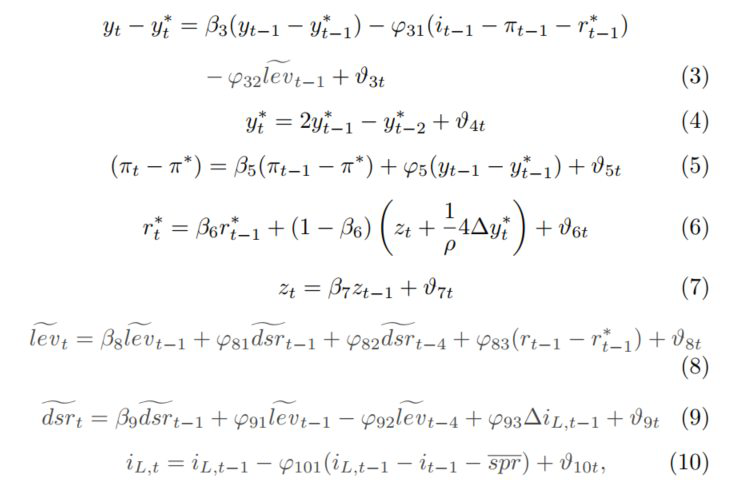
\includegraphics[scale=0.60]{LW_financial_cycles.png}
%\caption {\tiny Taxa Natural de Juros}
\end{figure}
%
%
\section{\citet{Kiley:2015}: What Can the Data Tell Us About the Equilibrium Real Interest Rate?}
LW bayesiano
Chegamos a duas conclusões principais. Primeiro, os dados fornecem relativamente pouca informação sobre o processo de geração de dados $r^{*}$; na verdade, a distribuição posterior desse processo está muito próxima da distribuição anterior. Estes resultados contrastam fortemente com os dos processos de tendência de crescimento ou taxa natural de desemprego, para os quais os dados são muito informativos. Em segundo lugar, os deslocadores de demanda adicionais - em particular, um spread de crédito - são muito importantes para as ligações estimadas entre o produto e as taxas de juros e, portanto, para as estimativas de $r^{*}$ - implicando que pesquisas anteriores que ignoram tais fatores fornecem inferência pobre. As estimativas de r ∗ que levam em conta essa gama de considerações são mais estáveis do que outras estimativas, com $r^{*}$ no final de 2014 igual a aproximadamente 1-1 / 4 por cento.
%
%
\section{\citet{Fries:2018}: National natural rates of interest and the single monetary policy in the euro area}

Neste artigo, estimamos as taxas de juros naturais nacionais variáveis no tempo para cada uma das quatro maiores economias da área do euro - França, Alemanha, Itália e Espanha - desde o início do euro em 1999. Filtramos essas variáveis não observadas condicionalmente em um modelo estilizado conjunto dessas quatro economias e suas interações. Encontramos primeiro evidências de uma tendência comum de declínio dos quatro r ∗ nacionais nos últimos 15 anos. Com exceção de alguns episódios de curta duração, sendo o último durante a recessão pós-Lehman, as diferenças no r national nacional entre os países permaneceram relativamente contidas e geralmente abaixo de 1 ponto percentual. No entanto, as taxas de juro reais de curto prazo (1 ano) divergiram acentuadamente durante a crise soberana da área do euro, reflectindo o aumento dos spreads de crédito soberano dos países do sul. Em seguida, calculamos as medidas específicas de cada país da diferença da taxa de juros real, a diferença entre a taxa real ex ante local e a taxa natural nacional estimada. De acordo com esta métrica, a política monetária única não foi comum entre os países membros ao longo de vários episódios, principalmente no clímax da crise na área do euro. Ao mesmo tempo em que garantiu uma postura neutra em relação às economias centrais, revelou-se fortemente desinflacionário na Espanha e na Itália de meados de 2011 ao final de 2012. Eventualmente, todos os quatro desvios das taxas de juros reais nacionais convergiram para cerca de -1\% ao longo dos anos de 2014 –2016, testemunhando uma orientação de política única mais consistente e expansionista em toda a área, à medida que o Eurosistema embarcou de forma mais decisiva em programas não convencionais.

Nossa estimativa produz valores plausíveis e significativos para todos os parâmetros-chave, especialmente as inclinações das curvas de Phillips e IS. Obtemos medidas variáveis no tempo das variáveis latentes não observadas no modelo: as taxas de juros naturais nacionais e os desvios das taxas de juros derivadas, os desvios do produto nacional e as taxas associadas de crescimento do produto potencial. Em primeiro lugar, descobrimos que as quatro taxas naturais nacionais flutuaram amplamente em torno de uma tendência global de declínio nos últimos 15 anos, um resultado consistente com as descobertas de Holston et al. (2016). As médias transversais de fato oscilavam entre 3,5\% em 2000 e -1,5\% em 2012, finalmente para atingir um nível próximo (mas abaixo) de zero em 2016. Antes da crise de 2008, r ∗ nacional também tendia a se mover cada vez mais, conforme a dispersão transversal diminuiu de -1,3\% em 2000 para -0,4\% em 2007. A crise financeira mundial desencadeada pelo colapso do Lehman Brothers e a recessão que se seguiu derrubou as taxas naturais em todos os quatro países, para cerca de -1\% . Embora tenham recuperado rapidamente depois disso, as suas trajetórias divergiram de novo em certa medida em 2010 e 2011. As taxas naturais nacionais permaneceram principalmente em território negativo durante a crise da dívida soberana da área do euro, atingindo um mínimo no segundo semestre de 2012, em quase -2\% em França e cerca de -1,5\% nos outros três países. Os r ∗ nacionais acabaram por se estabilizar em níveis ligeiramente negativos em todas as economias desde meados de 2015. Assim, uma vez que as taxas de juro reais reais de 1 ano divergiram acentuadamente durante a crise da área do euro, os desvios das taxas de juro nacionais estimados apontam para posturas de política monetária eficazes bastante diferenciadas nos quatro países ao longo dos anos 2011-2013. No geral, nossas estimativas sugerem que a política monetária única foi quase neutra na França no período pós-2009, enquanto
efeitos significativamente restritivos na Itália e Espanha em 2011-2012 e tem sido bastante expansionista na Alemanha desde 2013.

Contribuímos para três vertentes da literatura e debates políticos atuais. Primeiro, nosso estudo fornece uma ilustração de como usar o conceito de taxas de juros naturais para informar os formuladores de políticas. Em comparação com estudos anteriores, o nosso é o primeiro a estimar as taxas naturais para cada país membro da área do euro num enquadramento consistente. As nossas conclusões, portanto, lançam uma nova luz sobre o debate sobre a fragmentação financeira da área durante a década de 2010 e a relevância de uma política monetária "tamanho único" neste ambiente estressado caracterizado pelos choques amplamente assimétricos do pânico da dívida soberana.

Em segundo lugar, nossas estimativas de taxas de juros naturais para quatro grandes economias europeias também fornecem evidências úteis para o debate em curso sobre taxas reais baixas após a crise e a hipótese de estagnação secular.